%!TEX root = main.tex
\section{Synchronizability}\label{sec:criterion}

%In order to simplify the reasoning about the asynchronous semantics of a message passing system $\mathcal{S}$, 
We define a property called \emph{$k$-synchronizability}, for some $k>0$, which roughly, states that every execution of a message passing system $\mathcal{S}$ is ``equivalent'' to one which passes regularly through configurations where the message buffers are empty, and in between those configurations, the overall number of messages stored in the buffers is bounded by $k$ (where by ``equivalent'', we mean conflict-preserving permutation). We formalize this property as the equality between the set of traces generated by the asynchronous semantics and the set of traces generated by a particular semantics called \emph{$k$-synchronous} which allows precisely the kind of executions mentioned above.

\begin{figure}[t]
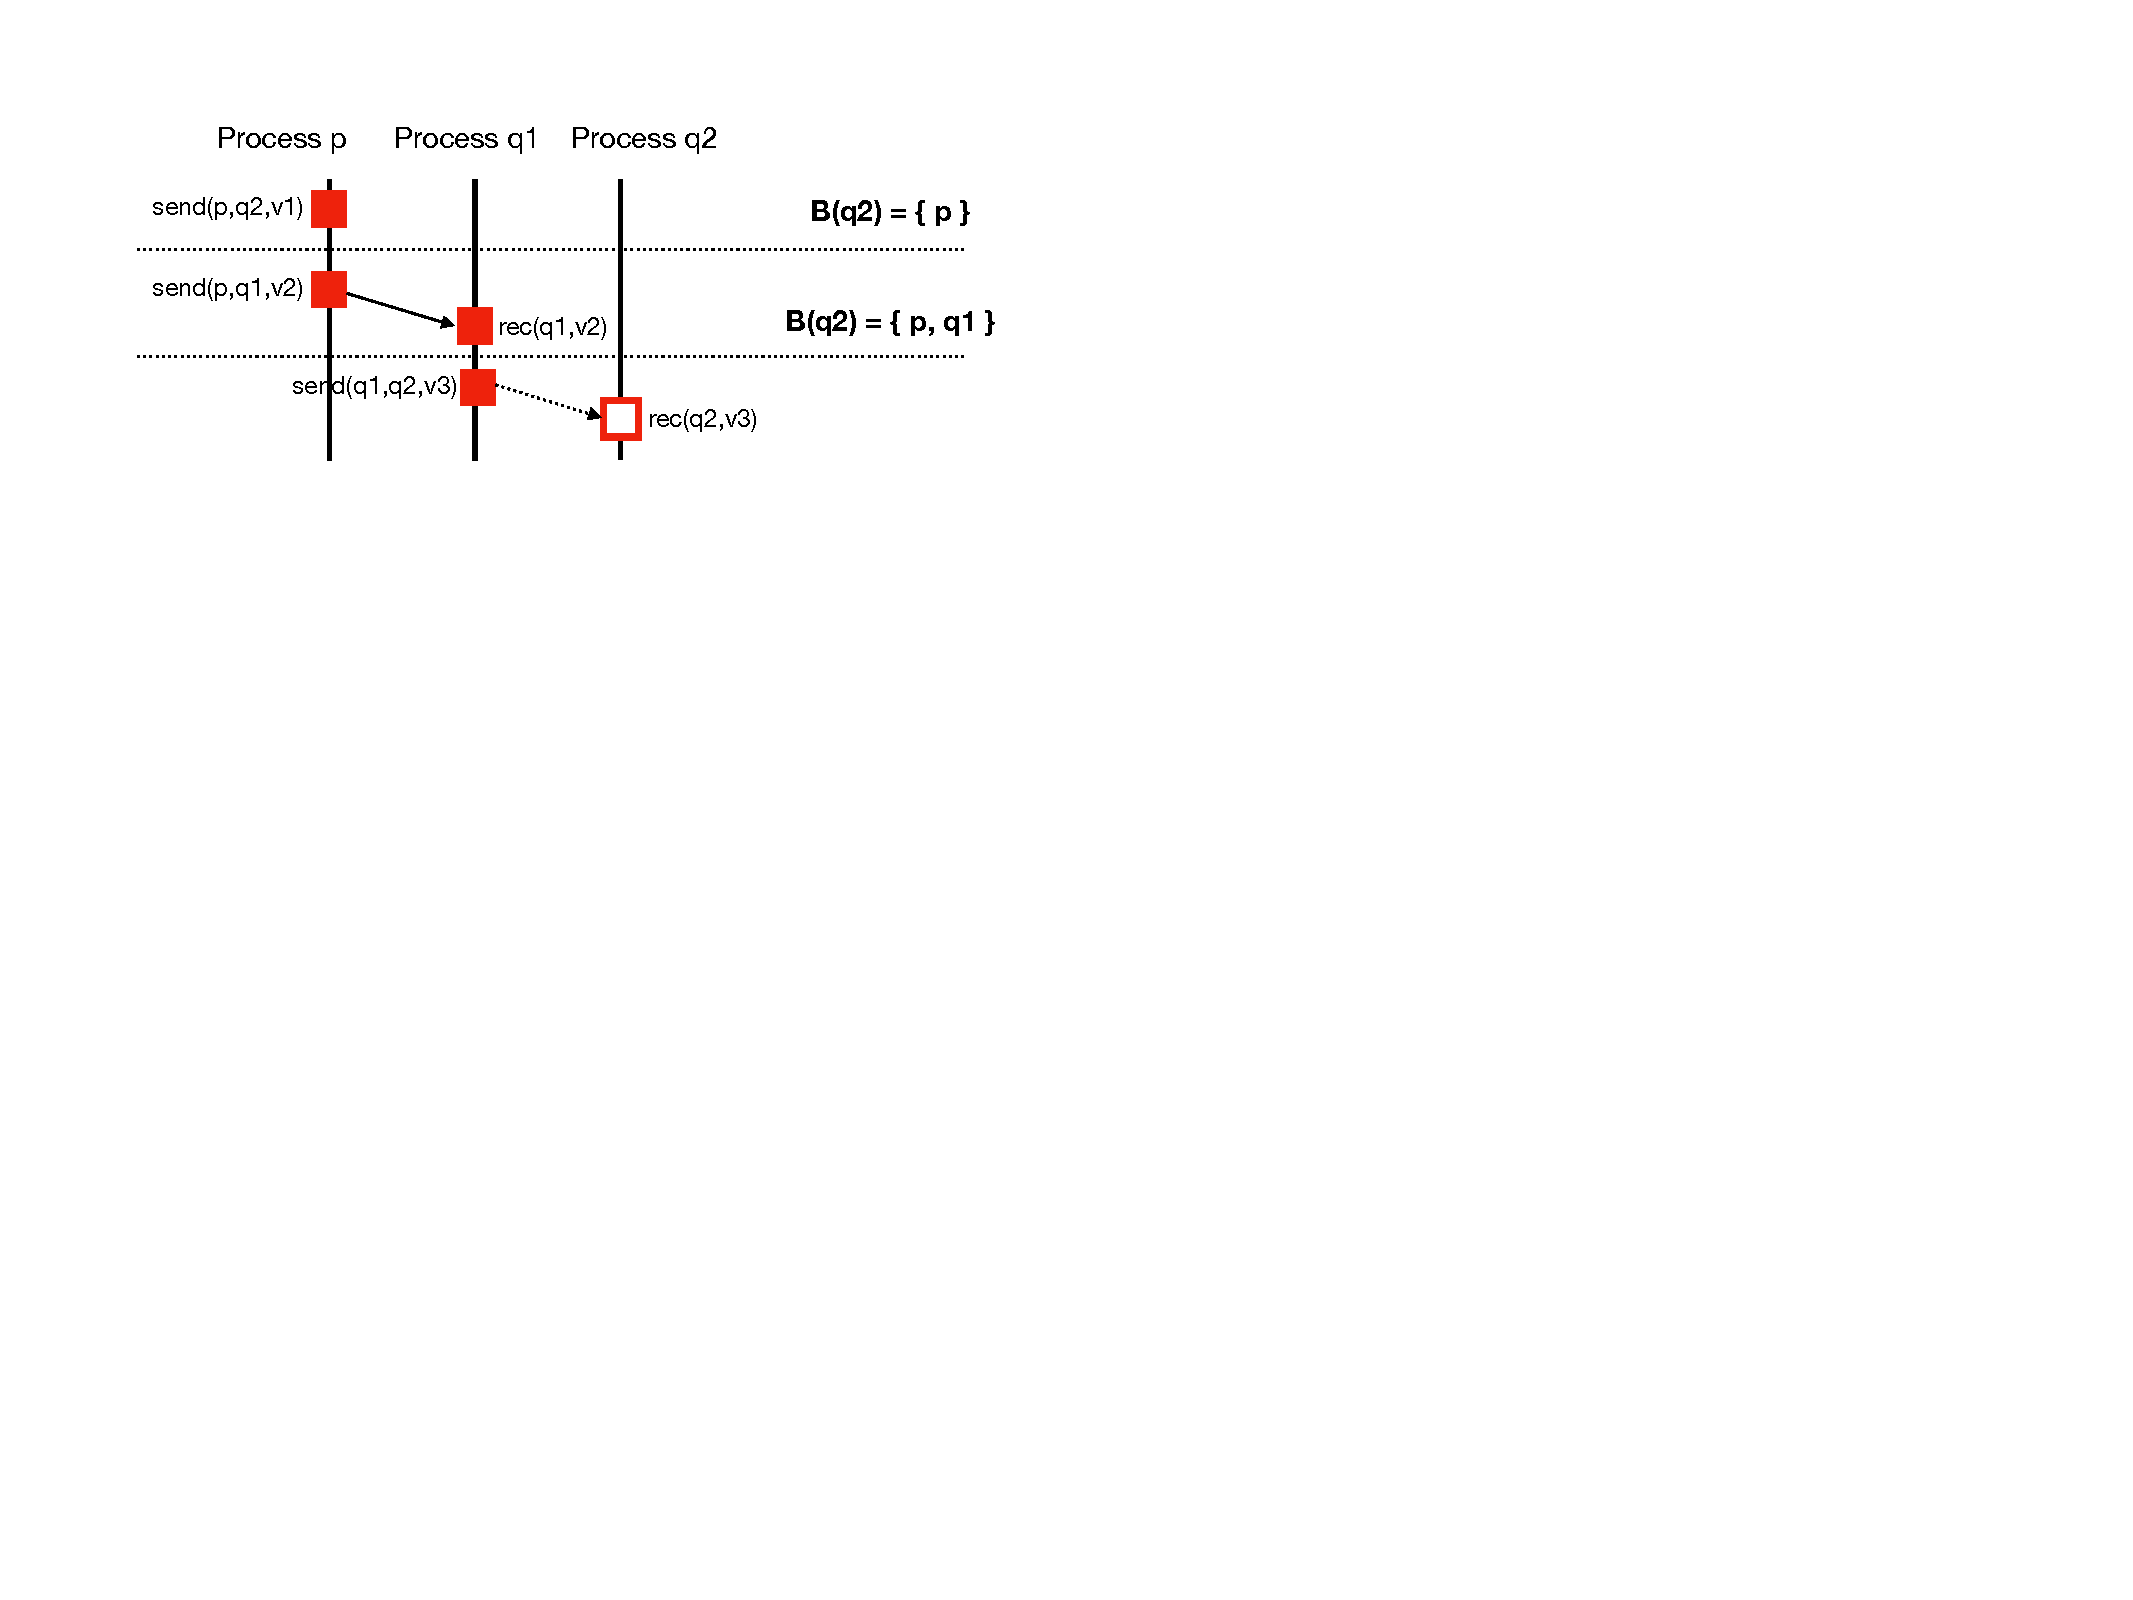
\includegraphics[width=8cm]{ex-blocking.pdf}
\caption{An execution of the $1$-synchronous semantics.}
\label{fig:ex-blocking}
\end{figure}

The $k$-synchronous semantics we define hereafter uses an extended version of the standard rendez-vous primitive where the message sent by a process is instantaneously received by the destination process. Roughly, in this extension, more than one process is allowed to send a message and a process can send multiple messages, but all these messages must be received before being allowed to send more messages. This primitive is called \emph{$k$-exchange} if the number of sent messages is smaller than $k$. Actually, to ensure that the $k$-synchronous semantics is prefix-closed (if it admits an execution, then it admits all its prefixes), we allow messages to be dropped during a $k$-exchange transition. For instance, the following execution 
\begin{align*}
\send{1}{p_1,q,\_}\ 
\send{2}{p_2,q,\_}\ 
\rec{1}{q,\_}\ 
\rec{2}{q,\_} 
\end{align*}
is an instance of a $2$-exchange and therefore admitted by the $2$-synchronous semantics. However, in order to ensure that the prefix without the last receive ($\rec{2}{q,\_}$) is also admitted, we allow $2$-exchange transitions to contain unmatched send actions. The presence of unmatched send actions must be constrained in order to ensure that the set of executions admitted by the $k$-synchronous semantics satisfies causal delivery. Consider for instance the execution in Figure~\ref{fig:ex-blocking} which can be produced by a sequence of $1$-exchanges. The receive action ($\reca{q_2,v_3}$) pictured as an empty box needs to be disabled in order to exclude violations of causal delivery. To this, the semantics tracks for each process $p$ a set of processes $B(p)$ from which it is forbidden to receive messages. Following the sequence of $1$-exchanges in this execution, the unmatched $\senda{p,q2,v1}$ disables any receive by $q2$ of a message sent by $p$ (otherwise, it will be even a violation of the FIFO semantics of $q2$'s buffer). Therefore, the first $1$-exchange results in $B(q2)=\{p\}$. The second $1$-exchange (the message from $p$ to $q1$) forbids $q2$ to receive any message from $q1$. Otherwise, this message will be necessarily causally related to $v1$, and receiving it will lead to a violation of causal delivery. Therefore, when reaching $\senda{q1,q2,v_3}$ the receive $\reca{q_2,v_3}$ is disabled because $q1\in B(q2)$.

%The standard rendez-vous primitive corresponds to the $1$-exchange. 
%The semantics allows messages to be dropped, but  TODO SAY THAT THIS IS RELATED TO AN IMPLICIT FIFO SEMANTICS FOR THE BUFFERS

\begin{figure} [t]
\footnotesize{
  \centering
  \begin{mathpar}
    \inferrule[$k$-exchange]{
      e\in S_{id}^*\cdot R_{id}^* \\ 
       |e| \leq 2\cdot k\\
%      \<msg>(a)\in [1,k]\mbox{ for every $a$ in $e$} \\
      (\vec{l},\vec{\epsilon})\xrightarrow{e} (\vec{l'},\vec{b}),\mbox{ for some $\vec{b}$}\\
            \forall s,r\in e.\ s\match r\implies\<proc>(s)\not\in B(\<dest>(s)) \\
       B'(q) = B(q) \cup \{p: \exists s\in e\cap S_{id}.\ ((\not\exists r\in e.\ s\match r)\land p = \<proc>(s)\land q=\<dest>(s)) \lor (\<proc>(s)\in B(q)\land \<dest>(s) = p)\}
    }{
      (\vec{l},B)
      \xRightarrow{e}{_k}
      (\vec{l'},B')
    }%\hspace{5mm}
    
%    \inferrule[drop]{
%      l\in \delta_p(\vec{l}_p,\senda{p,q,v}) \neq \emptyset
%    }{
%      (\vec{l},F)
%      \xRightarrow{\senda{p,q,v}}{_k}
%      (\vec{l}[\vec{l}_p\gets l],F\cup \{q\})
%    }%\hspace{5mm}
    
%    \inferrule[local]{ 
%      l\in \delta(\vec{l}_p,\epsilon) \neq \emptyset
%    }{
%      \vec{l},\vec{b}
%      \xrightarrow{\epsilon}
%      \vec{l}[\vec{l}_p\gets l],\vec{b}
%    }%\hspace{5mm}
  \end{mathpar}
  }
% \vspace{-5mm}
  \caption{The synchronous semantics of a message passing system $\mathcal{S}$. Above, $\vec{\epsilon}$ denotes a vector where all the components are $\epsilon$.
  %and for a sequence of indexed actions $e\in(S_{id}\cup R_{id})^*$, $\overline{e}$ denotes the sequence of \emph{actions} obtained from $e$ by removing message identifiers.
  %$\vec{b}[\vec{b}_q.\ \mathrm{add}(m)]$ denotes the vector of message buffers obtained from $\vec{b}$ by calling the method $\mathrm{add}(m)$ of the element of index $q$.
  }
  \label{fig:synch-sem}
%\vspace{-6mm}
\end{figure}

Formally, a configuration $c'=(\vec{l},B)$ in the synchronous semantics is a vector $\vec{l}$ of local states together with a function $B:\<Pids>->2^{\<Pids>}$. The transition relation $\Rightarrow_k$ is defined in Figure~\ref{fig:synch-sem}. A \textsc{$k$-exchange} transition corresponds to a sequence of transitions of the asynchronous semantics starting from a configuration with empty buffers. The sequence of transitions is constrained to be a sequence of at most $k$ sends followed by a sequence of receives. The receives are enabled depending on previous unmatched sends as explained above, using the function $B$.
The semantics defined by $\Rightarrow_k$ is called the $k$-synchronous semantics.

Executions and traces are defined as in the case of the asynchronous semantics, using $\Rightarrow_k$ for some fixed $k$ instead of $\rightarrow$. The set of executions, resp., traces, of $\mathcal{S}$ under the $k$-synchronous semantics is denoted by $\synchExec{\mathcal{S}}{k}$, resp., $\synchTr{\mathcal{S}}{k}$. The executions in $\synchExec{\mathcal{S}}{k}$ and the traces in 
$\synchTr{\mathcal{S}}{k}$ are called $k$-synchronous. 

%A trace $t\in \synchTr{\mathcal{S}}{k}$, for some $\mathcal{S}$, is called $k$-synchronous. 
An execution $e$ such that $tr(e)$ is $k$-synchronous is called $k$-synchronizable. We omit $k$ when it is not important. 

For a given system $\mathcal{S}$, the set of executions generated by $\mathcal{S}$ under the $k$-synchronous semantics is prefix-closed. Therefore, the set of $k$-synchronizable executions of a system $\mathcal{S}$ is also prefix-closed.

\begin{lemma}\label{lem:pref_closed}
For a system $\mathcal{S}$, let $e\in\asynchExec{\mathcal{S}}$ be a $k$-synchronizable execution. Then, every prefix of $e$ is $k$-synchronizable. 
\end{lemma}
%\begin{proof}
%%We have to show that every cycle in a prefix $e'$ of $e$ is good and of size at most $k$. 
%Since the conflict graph $CG_{tr(e')}$ is a subgraph of $CG_{tr(e)}$, every cycle in $CG_{tr(e')}$ occurs also in $CG_{tr(e)}$. Therefore, since all the cycles of $e$ are good and of size at most $k$, the same holds for all the cycles in $e'$.
%\end{proof}

As a direct consequence of Lemma~\ref{lem:undist}, we get that $k$-synchronizable and $k$-synchronous executions are undistinguishable up to conflict-preserving permutations.

\begin{lemma}\label{lem:zable_nous}
For every $k$-synchronizable execution $e$, there exists a permutation $e'$ of $e$ which is $k$-synchronous.
\end{lemma}


\begin{definition}\label{def:synchron}
A message passing system $\mathcal{S}$ is called \emph{$k$-synchronizable} when $\asynchTr{\mathcal{S}}=\synchTr{\mathcal{S}}{k}$.
\end{definition}

%As a consequence of Definition~\ref{def:synchron}, a system $\mathcal{S}$ is not $k$-synchronizable when it admits an execution $e$ (under the asynchronous semantics) which is not $k$-synchronous (i.e., its trace is not $k$-synchronous). Such an execution $e$ is called a \emph{violation to $k$-synchronizability}.

The following result shows that $k$-synchronizable systems reach exactly the same set of local state vectors under the asynchronous and the $k$-synchronous semantics. Therefore, any assertion checking or invariant checking problem for a $k$-synchronizable system $\mathcal{S}$ can be solved by considering the $k$-synchronous semantics instead of the asynchronous one. In particular, this implies that such problems are decidable for finite-state $k$-synchronizable systems~\footnote{A system is called \emph{finite-state} when the number of local states of every process is bounded.} whereas they are undecidable for arbitrary systems. The $k$-synchronous semantics of a finite-state system can be modeled by a finite-state labeled transition system since the message buffers are of bounded size.

\begin{theorem}
For a $k$-synchronizable message passing system $\mathcal{S}$, $\asynchSt{\mathcal{S}}=\synchSt{\mathcal{S}}{k}$.
\end{theorem}
\begin{proof}
Direct consequence of Lemma~\ref{lem:undist}.
\end{proof}

Appendix~\ref{asec:deadlocks} shows that the problem of detecting deadlocks in a $k$-synchronizable system can also be solved using the $k$-synchronous semantics instead of the asynchronous one

